%%%%%%%%%%%%%%%%%%%%%%%%%%%%%%%%%%%%%%%%%
% Programming/Coding Assignment
% LaTeX Template
%
% This template has been downloaded from:
% http://www.latextemplates.com
%
% Original author:
% Ted Pavlic (http://www.tedpavlic.com)
%
% Note:
% The \lipsum[#] commands throughout this template generate dummy text
% to fill the template out. These commands should all be removed when 
% writing assignment content.
%
% This template uses a Perl script as an example snippet of code, most other
% languages are also usable. Configure them in the "CODE INCLUSION 
% CONFIGURATION" section.
%
%%%%%%%%%%%%%%%%%%%%%%%%%%%%%%%%%%%%%%%%%

%----------------------------------------------------------------------------------------
%	PACKAGES AND OTHER DOCUMENT CONFIGURATIONS
%----------------------------------------------------------------------------------------

\documentclass{article}

\usepackage{fancyhdr} % Required for custom headers
\usepackage{lastpage} % Required to determine the last page for the footer
\usepackage{extramarks} % Required for headers and footers
\usepackage[usenames,dvipsnames]{color} % Required for custom colors
\usepackage{graphicx} % Required to insert images
\usepackage{listings} % Required for insertion of code
\usepackage{courier} % Required for the courier font
\usepackage{lipsum} % Used for inserting dummy 'Lorem ipsum' text into the template
\usepackage{url}
\newcommand{\quotes}[1]{``#1''}
% Margins
\topmargin=-0.45in
\evensidemargin=0in
\oddsidemargin=0in
\textwidth=6.5in
\textheight=9.0in
\headsep=0.25in

\linespread{1.1} % Line spacing

% Set up the header and footer
\pagestyle{fancy}
\lhead{\hmwkAuthorName} % Top left header
\chead{\hmwkClass\ (\hmwkClassInstructor\ \hmwkClassTime) \hmwkTitle} % Top center head
\rhead{\firstxmark} % Top right header
\lfoot{\lastxmark} % Bottom left footer
\cfoot{} % Bottom center footer
\rfoot{Page\ \thepage\ of\ \protect\pageref{LastPage}} % Bottom right footer
\renewcommand\headrulewidth{0.4pt} % Size of the header rule
\renewcommand\footrulewidth{0.4pt} % Size of the footer rule

\setlength\parindent{0pt} % Removes all indentation from paragraphs

%----------------------------------------------------------------------------------------
%	CODE INCLUSION CONFIGURATION
%----------------------------------------------------------------------------------------

\definecolor{MyDarkGreen}{rgb}{0.0,0.4,0.0} % This is the color used for comments
\lstloadlanguages{R} % Load Perl syntax for listings, for a list of other languages supported see: ftp://ftp.tex.ac.uk/tex-archive/macros/latex/contrib/listings/listings.pdf
\lstset{language=R, % Use Perl in this example
        frame=single, % Single frame around code
        basicstyle=\small\ttfamily, % Use small true type font
        keywordstyle=[1]\color{Blue}\bf, % Perl functions bold and blue
        keywordstyle=[2]\color{Purple}, % Perl function arguments purple
        keywordstyle=[3]\color{Blue}\underbar, % Custom functions underlined and blue
        identifierstyle=, % Nothing special about identifiers                                         
        commentstyle=\usefont{T1}{pcr}{m}{sl}\color{MyDarkGreen}\small, % Comments small dark green courier font
        stringstyle=\color{Purple}, % Strings are purple
        showstringspaces=false, % Don't put marks in string spaces
        tabsize=5, % 5 spaces per tab
        %
        % Put standard Perl functions not included in the default language here
        morekeywords={},
        %
        % Put Perl function parameters here
        morekeywords=[2]{on, off, interp},
        %
        % Put user defined functions here
        morekeywords=[3]{test},
       	%
        morecomment=[l][\color{Blue}]{...}, % Line continuation (...) like blue comment
        numbers=left, % Line numbers on left
        firstnumber=1, % Line numbers start with line 1
        numberstyle=\tiny\color{Blue}, % Line numbers are blue and small
        stepnumber=5 % Line numbers go in steps of 5
}

% Creates a new command to include a perl script, the first parameter is the filename of the script (without .pl), the second parameter is the caption
\newcommand{\rscript}[2]{
\begin{itemize}
\item[]\lstinputlisting[caption=#2,label=#2]{#1.R}
\end{itemize}
}

%----------------------------------------------------------------------------------------
%	DOCUMENT STRUCTURE COMMANDS
%	Skip this unless you know what you're doing
%----------------------------------------------------------------------------------------

% Header and footer for when a page split occurs within a problem environment
\newcommand{\enterProblemHeader}[1]{
\nobreak\extramarks{#1}{#1 continued on next page\ldots}\nobreak
\nobreak\extramarks{#1 (continued)}{#1 continued on next page\ldots}\nobreak
}

% Header and footer for when a page split occurs between problem environments
\newcommand{\exitProblemHeader}[1]{
\nobreak\extramarks{#1 (continued)}{#1 continued on next page\ldots}\nobreak
\nobreak\extramarks{#1}{}\nobreak
}

\setcounter{secnumdepth}{0} % Removes default section numbers
\newcounter{homeworkProblemCounter} % Creates a counter to keep track of the number of problems

\newcommand{\homeworkProblemName}{}
\newenvironment{homeworkProblem}[1][Problem \arabic{homeworkProblemCounter}]{ % Makes a new environment called homeworkProblem which takes 1 argument (custom name) but the default is "Problem #"
\stepcounter{homeworkProblemCounter} % Increase counter for number of problems
\renewcommand{\homeworkProblemName}{#1} % Assign \homeworkProblemName the name of the problem
\section{\homeworkProblemName} % Make a section in the document with the custom problem count
\enterProblemHeader{\homeworkProblemName} % Header and footer within the environment
}{
\exitProblemHeader{\homeworkProblemName} % Header and footer after the environment
}

\newcommand{\problemAnswer}[1]{ % Defines the problem answer command with the content as the only argument
\noindent\framebox[\columnwidth][c]{\begin{minipage}{0.98\columnwidth}#1\end{minipage}} % Makes the box around the problem answer and puts the content inside
}

\newcommand{\homeworkSectionName}{}
\newenvironment{homeworkSection}[1]{ % New environment for sections within homework problems, takes 1 argument - the name of the section
\renewcommand{\homeworkSectionName}{#1} % Assign \homeworkSectionName to the name of the section from the environment argument
\subsection{\homeworkSectionName} % Make a subsection with the custom name of the subsection
\enterProblemHeader{\homeworkProblemName\ [\homeworkSectionName]} % Header and footer within the environment
}{
\enterProblemHeader{\homeworkProblemName} % Header and footer after the environment
}

%----------------------------------------------------------------------------------------
%	NAME AND CLASS SECTION
%----------------------------------------------------------------------------------------

\newcommand{\hmwkTitle}{Homework\ \#2} % Assignment title
\newcommand{\hmwkDueDate}{Friday, Feb 9,  2018 10:00 p.m.}% Due date
\newcommand{\hmwkClass}{Introduction to Data Analysis and Mining\\} % Course/class
\newcommand{\hmwkClassTime}{MW 6:00pm} % Class/lecture time
\newcommand{\hmwkClassInstructor}{Instructor: Hasan Kurban} % Teacher/lecturer
\newcommand{\hmwkAuthorName}{Siyi Xian} % Your name

%----------------------------------------------------------------------------------------
%	TITLE PAGE
%----------------------------------------------------------------------------------------

\title{
\vspace{2in}
\textmd{\textbf{\hmwkClass\ \hmwkTitle}}\\
\normalsize\vspace{0.1in}\small{Due\ on\ \hmwkDueDate}\\
\vspace{0.1in}\large{\textit{\hmwkClassInstructor\ }}
\vspace{3in}
}

\author{\textbf{\hmwkAuthorName}}
\date{\today} % Insert date here if you want it to appear below your name

%----------------------------------------------------------------------------------------

\begin{document}

\title{ CSCI-B 365 Introduction to Data Analysis and Mining\\
Homework 2 \\
Computer Science \\
Spring 2018 \\Indiana University,\\ Bloomington, IN}
\author{ Siyi Xian \\ siyixian@indiana.edu}
\date{ Friday, Feb 9,  2018 10:00 p.m. }
\maketitle
All the work herein is solely mine.

\maketitle

%----------------------------------------------------------------------------------------
%	TABLE OF CONTENTS
%----------------------------------------------------------------------------------------

%\setcounter{tocdepth}{1} % Uncomment this line if you don't want subsections listed in the ToC

\newpage
\tableofcontents
\newpage

%----------------------------------------------------------------------------------------
%	PROBLEM 1
%----------------------------------------------------------------------------------------

\begin{homeworkProblem} 

Textbook exercises, chapter 2, pages: 91-93
\begin{enumerate}
\item Exercise 12  \textbf{(10 points)}
\begin{verbatim}
(a) Noise is not, but outliers are.

(b) Noise objects can be outliers, because the original values can be 
    modified to values which are far away from mainly data range.
    
(c) Noise objects are not always outliers, because original values
    can be modified to some values that are similar to correct data.
    
(d) Outliers are not always noise. They are mainly be a set of data 
    which is a lot more different than others.
    
(e) Yes

\end{verbatim}
\item Exercise 15  \textbf{(10 points)}
\begin{verbatim}
For the first scheme, the data get from the set is exactly the same 
in each group. However, the second scheme, the amount from each group 
is only roughly the same.

\end{verbatim}
\item Exercise 16  \textbf{(10 points)}
\begin{verbatim}
(a) Words that appear in every documents, weight will be too small. 
    Otherwise, the weight will be extremely high.
    
(b) To distinguish documents from each others which the original data 
    cannot observe the similarity. 
    
\end{verbatim}
\item Exercise 18  \textbf{(15 points)}
\begin{verbatim}
(a) Hamming distance   = number of different bits 
                       = 3
    Jaccard Similarity = "1-1" matches /(bits - "0-0" matches) 
                       = 2 / 5 
                       = 0.4

(b) The Hamming distance is similar to the Simple Matching Coefficient, 
    because SMC = Hamming distance / number of bits.
    The Jaccard Similarity is similar to the cosine 
    because both of them does not consider "0-0" matches.
\end{verbatim}
\clearpage
\begin{verbatim}
(c) Jaccard is better for comparing how similar two organisms of 
    different species. The reason is that the result we want to find 
    is how many genes are in common for different species.
    
(d) Hamming distance is better to compare genetic makeup of two organisms 
    of the same species, because for the same species, most of their genes 
    are the same. So, it is only necessary to compare the differences.

\end{verbatim}
\item Exercise 19  \textbf{(15 points)}
\begin{verbatim}
(a) cos(x, y) = 1
    corr(x, y): undefined
    Euclidean(x, y) = 2
    
(b) cos(x, y) = 0
    corr(x, y) = ?1
    Euclidean(x, y) = 2
    Jaccard(x, y) = 0
    
(c) cos(x, y) = 0
    corr(x, y)=0
    Euclidean(x, y) = 2
    
(d) cos(x, y) = 0.75
    corr(x, y) = 0.25
    Jaccard(x, y) = 0.6
    
(e) cos(x, y) = 0
    corr(x, y) = 0

\end{verbatim}
\end{enumerate}
\end{homeworkProblem}
\clearpage


%----------------------------------------------------------------------------------------
%	PROBLEM 2
%----------------------------------------------------------------------------------------

% To have just one problem per page, simply put a \clearpage after each problem


\begin{homeworkProblem} 
For the following data, give the best taxonomic type (interval, ratio, nominal, ordinal):
\begin{enumerate}
\item A section of highway on a map.
\begin{verbatim}
Highway on a map is a nominal data, because different name of highways 
represent different high ways. For example I-45 is a different highway 
with I-37, and both of them are unique highways.
\end{verbatim}
\item The value of a stock.
\begin{verbatim}
Stock is a ratio data. Difference can show the profit or loss, and ratio
can show changes between weeks, months, or years.
\end{verbatim}
\item The weight of a person.
\begin{verbatim}
Weight can be a ordinal data which can be a sorting standers for people.
\end{verbatim}
\item Marital status.
\begin{verbatim}
Marital status is a nominal data which can distinguish people in to
couple of groups.
\end{verbatim}
\item Visiting United Airlines (\url{https://www.united.com}) the seating is: Economony, Economy plus, and United Business.  
\begin{verbatim}
Seating is a nominal data which can distinguish people in to couple 
of groups.
\end{verbatim}
\textbf{(10 points: each question is worth 2 points)}
\end{enumerate}
\end{homeworkProblem}
\clearpage

%----------------------------------------------------------------------------------------
%	PROBLEM 3
%----------------------------------------------------------------------------------------


\begin{homeworkProblem}
You are datamining with a column that has physical addresses in some city with the same zipcode.  For example,
\begin{verbatim}

55 WEST CIR
2131 South Creek Road
Apt. #1 Fountain Park
1114 Rosewood Cir
1114 Rosewood Ct.
1114 Rosewood Drive

\end{verbatim}

What structure would you create to mine these?  What questions do you think you should be able to answer?  \textbf{(10 points)}
\begin{verbatim}
Road Name -> Road Type (Ct., Dr, Ln, and etc.) ->  House Number -> Apartment Number
\end{verbatim}
\end{homeworkProblem}
\clearpage

%----------------------------------------------------------------------------------------
%	PROBLEM 4
%----------------------------------------------------------------------------------------


\begin{homeworkProblem}
The Wisconsin Breast Cancer data set is very famous. Here is the URL \url{https://archive.ics.uci.edu/ml/datasets/breast+cancer+wisconsin+(original)}.  In the Data Folder are multiple files.  Here is the beginning of an R session that allows us to read this data from the web into our local R session:
\begin{verbatim}
> install.packages("data.table")
> library(data.table)
> install.packages("curl")
> mydata <- fread("https://archive.ics.uci.edu/ml/machine-learning-databases/
                   breast-cancer-wisconsin/breast-cancer-wisconsin.data")
> head(mydata)
        V1 V2 V3 V4 V5 V6 V7 V8 V9 V10 V11
1: 1000025  5  1  1  1  2  1  3  1   1   2
2: 1002945  5  4  4  5  7 10  3  2   1   2
3: 1015425  3  1  1  1  2  2  3  1   1   2
4: 1016277  6  8  8  1  3  4  3  7   1   2
5: 1017023  4  1  1  3  2  1  3  1   1   2
6: 1017122  8 10 10  8  7 10  9  7   1   4
> 
\end{verbatim}
\subsection{Discussion of Data}
Briefly describe this data set--what is its purpose?  How should it be used? What are the kinds of data it's using?
\begin{verbatim}
Samples arrive periodically as Dr. Wolberg reports his clinical cases.
The database therefore reflects this chronological grouping of the data.
The database are using the result of experientment. 
\end{verbatim}
\subsection{R Code}
 Using R, show code that answers the following questions:
\begin{enumerate} 
\item How many entries are in the data set? $699$


\rscript{HW2-4-1}{Entries}

\item How many unknown or missing data are in the data set? $16$
\rscript{HW2-4-2}{Missing Data}
\item How many malignant and benign identifiers are there? $Malignant: 241$  $Benign: 458$
\rscript{HW2-4-3}{Malignant and Benign}
\item Make a histogram of each attribute and discuss the distribution of values \textit{e.g.}, are uniform, skewed, normal.  Place images of these histograms into the document.   Show the R code that you used below and discussion below that. 
\rscript{HW2-4-4}{Histogram}
\subsection{Discussion of Attributes}
$Positive$ $Skewed$
\subsection{Histograms}
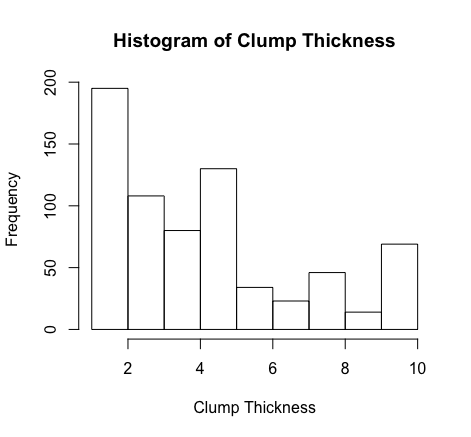
\includegraphics[width=8cm]{2.png}
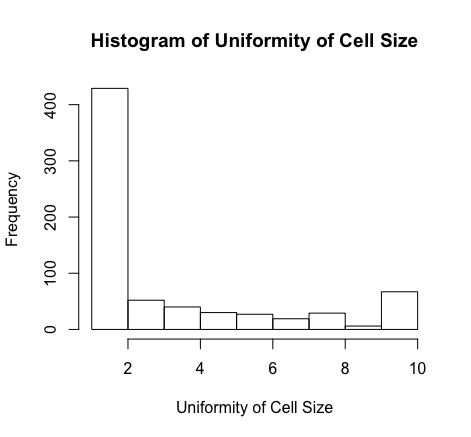
\includegraphics[width=8cm]{3.png} 
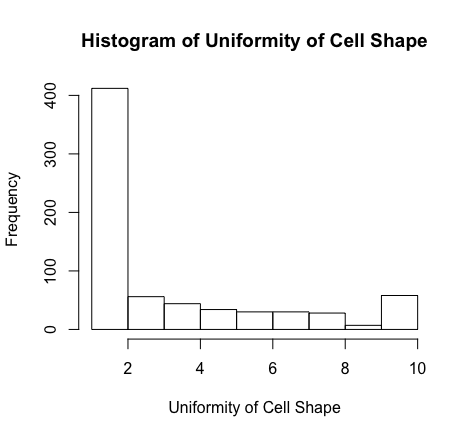
\includegraphics[width=8cm]{4.png} 
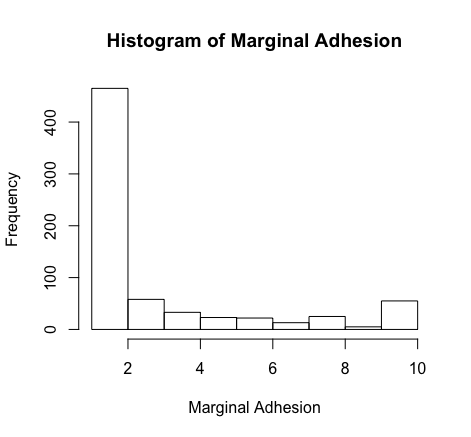
\includegraphics[width=8cm]{5.png} 
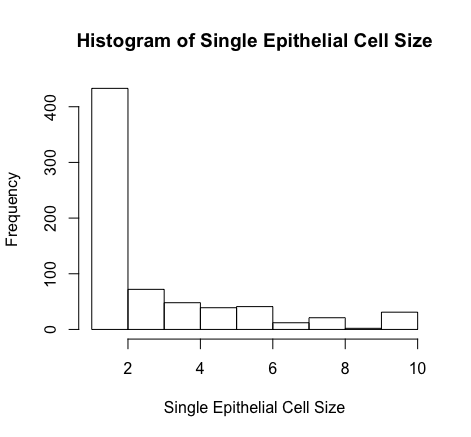
\includegraphics[width=8cm]{6.png} 
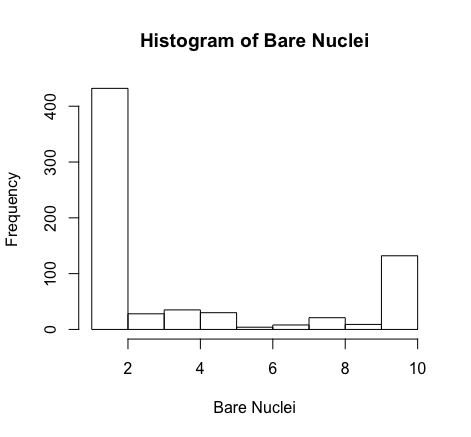
\includegraphics[width=8cm]{7.png} 
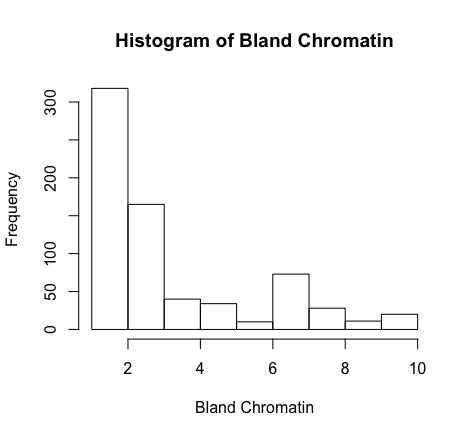
\includegraphics[width=8cm]{8.png}
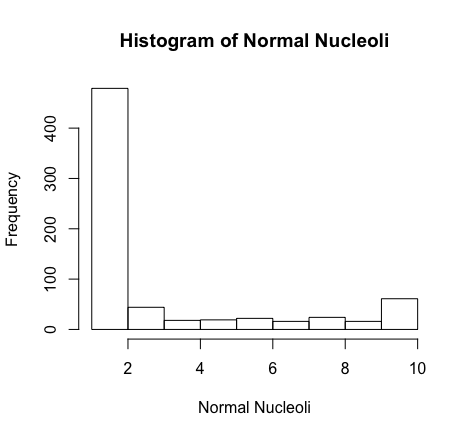
\includegraphics[width=8cm]{9.png} 
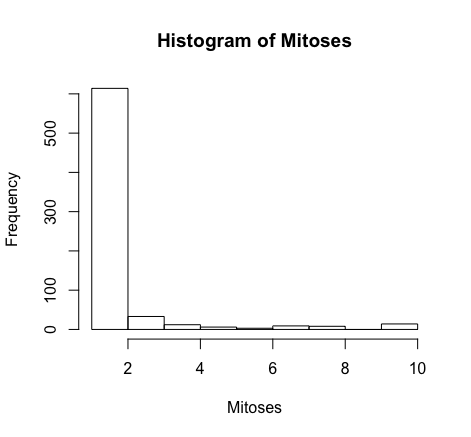
\includegraphics[width=8cm]{10.png} 
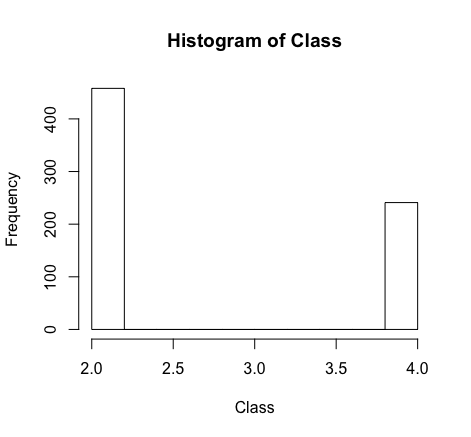
\includegraphics[width=8cm]{11.png} 
\end{enumerate} 
\subsection{Discussion of simply removing tuples}
Quantify the affect of simply removing the tuples with unknown or missing values.  What is the cost in human capital?  \textbf{(20 points)}
\begin{verbatim}
When simply removing those tuples, the other information the contains in the 
tuple that are not missing are gave up either. So it will waste a lot by 
doing that.
\end{verbatim}
\end{homeworkProblem}
\clearpage

%----------------------------------------------------------------------------------------

\section*{What to Turn-in }
Please follow the syllabus guidelines in turning in your homework.  I am providing the \LaTeX{} of this document too. This homework is due Friday, Feb  9, 2018 10:00p.m. \textbf{OBSERVE THE  TIME}. Absolutely no homework will be accepted after that time. 
All the work should be your own.   Submit a .zip file that includes the files below. Name the .zip as \quotes{usename-section number}, i.e., hakurban-B365.
\begin{enumerate}
\item The *tex and *pdf of the written answers to this document.
\end{enumerate}

%----------------------------------------------------------------------------------------

\end{document}